\section{Main simulation panel}
    This panel is the main part of the simulator user interface. Simulator mimics functionality of PicoBlaze instruction
    set and provide detailed view in its registers, overview of input and output ports, etc., and displays warning when
    the simulated program behaves strangely i.e. does something which under normal circumstances results an error.
    Following picture shows main window of the simulator. You can find here internal registers, scratch-pad ram, input
    and output ports, stack, program counter, elapsed time and cycles, current clock and internal flags: CARRY and ZERO.
    All those features can be edited during processor simulation. If some value changes state, it will turn yellow. You
    can drag out whole simulation panel and place outside of the main window, for example another display/monitor on
    your computer.

   \begin{figure}[h!]
        \centering
        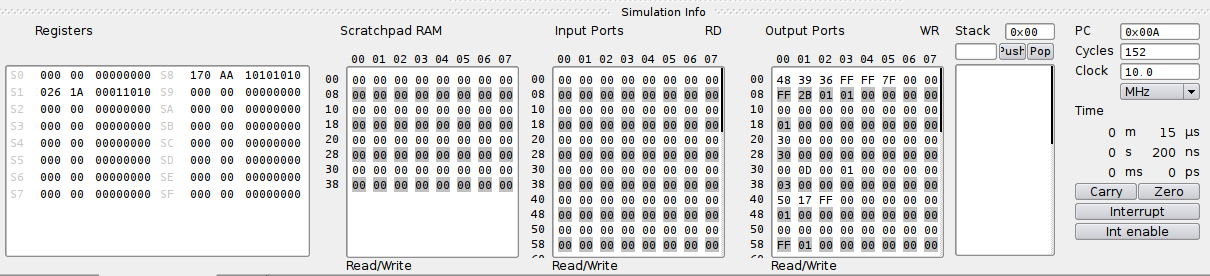
\includegraphics[width=\textwidth]{img/bottom_panel.png}
        \caption{Main simulator panel}
    \end{figure}

    \begin{description}
        \item [Registers]
            You can find here values of internal processor registers. The first column represents name, second value in
            decimal, third hexadecimal value, and last binary value.
        \item [Scratch-pad RAM]
            This hexadecimal editor represents values stored in the scratch-pad RAM. Address of a particular field is
            addition of the line and column numbers.
        \item [Ports]
            Output and input ports are represented by hex editors in full their address range. Besides viewing and
            changing input and output values, you can also see the status of PicoBlaze RD and WR signals. It can be
            useful for easier debugging.
        \item [Stack]
            Stack window represents values stored in stack. You can change the stack content by pushing and popping
            values, and view its virtual stack pointer.
        \item [Info panel]
            Panel on the right side of simulation panel gives you general information about simulated code. You can find
            there the program counter, number of executed cycles, clock frequency, elapsed time and status flags Carry
            and Zero, plus normally hidden Interrupt Enable flag. You can also invoke an interrupt by clicking on the
            Interrupt button. Buttons showing status flags or other flags can also change them (click on such button to invert the flag). Green text in ``flag button'' indicates that the flag is set to 1, black text indicates that value of the flag is 0.
    \end{description}

    \subsection{Simulator warnings}
        The simulator can display several warnings to handle some common mistakes in software development like program counter overflow, stack overflow, and some others; it is meant to make your debugging process less painful. Please see pictures bellow for more information, or go to
        [Main~Menu] -> [Interface] -> [Config] -> [Simulator~warnings] in the main window.

        \begin{table}[h!]
            \begin{tabular}{cc}
                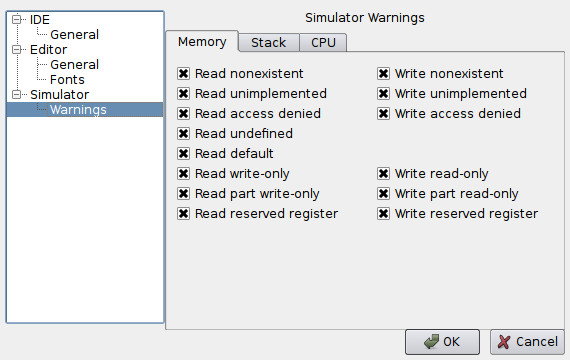
\includegraphics[width=.45\textwidth]{img/interface4.png}
                    &
                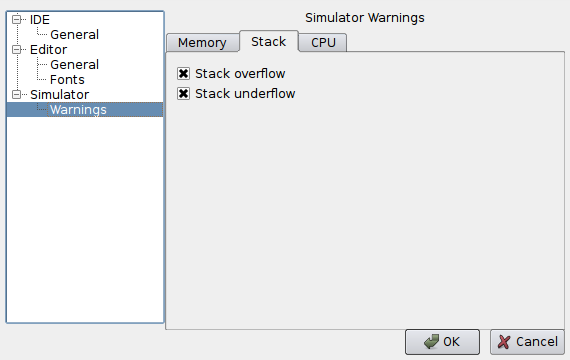
\includegraphics[width=.45\textwidth]{img/interface5.png}
                \\ Simulator -> Warnings -> Memory & Simulator -> Warnings -> Stack
                \\
                \\ 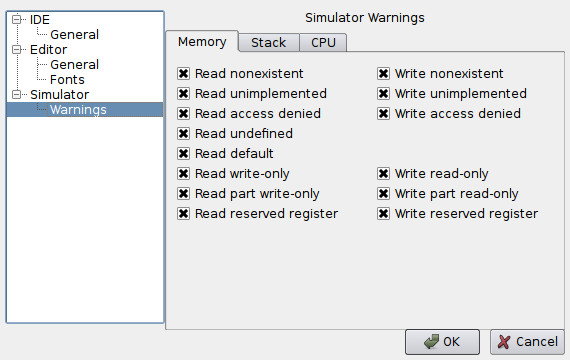
\includegraphics[width=.5\textwidth]{img/interface4.png}
                \\ Simulator -> Warnings -> CPU
            \end{tabular}
        \end{table}

    \subsection{Breakpoints and bookmarks}
        \begin{wrapfigure}{r}{0pt}
            \centering
                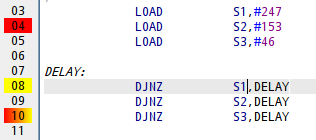
\includegraphics[width=.35\textwidth]{img/breakpoints1.png}
                \caption{Yellow - bookmark, Red - breakpoint, Yellow/Red gradient - both}
        \end{wrapfigure}
        MDS simulator supports breakpoints, breakpoint is a mark associated with a location in the program code; when
        reached, it triggers a temporarily halt in the running simulation. You can use breakpoints to test and debug
        programs in a manner that the program can be examined in stages delimited by breakpoints. Please be also aware
        that using breakpoints slows down the simulator; if you want maximum simulation speed, you may temporarily
        disable (switch off) breakpoints generally in [Main~Menu]~-> [Simulation]~-> [Disable~Breakpoints].

        Another feature is bookmarks; when editing one location in your source code more often, it may be useful to add
        a bookmark to it so you can quickly get back when you need. Like breakpoints bookmarks are marks in your source
        code but they are meant solely for quick navigation, they do not affect simulation in any way.

    \subsection{Simulation cursor}
        Simulation cursor shows what instruction will be executed in next step. Two previous instructions are less and
        less highlighted, so you can track two previous steps. following figure displays actual cursor on line 8, one
        step before is on line 5 and another step is on 4.
        \begin{figure}[h!]
            \centering
            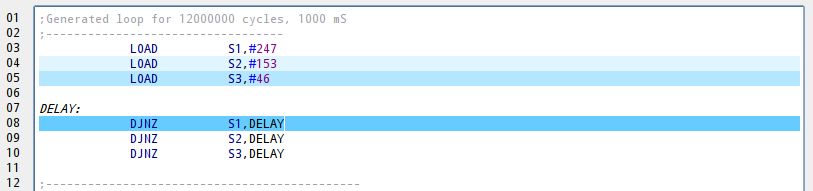
\includegraphics[width=\textwidth]{img/simulationcursor1.png}
            \caption{Simulation cursor}
        \end{figure}

        When simulator encounters macro expansion, for better orientation, cursor will appear on two or more locations.
        On macro expansion and in macro definition, showing what is being executed and where it came from. When you have
        macro expanded in another macro, you will see three cursors and so on. For better understanding, the following
        figure shows simulation cursor behavior with macros.
        \begin{figure}[h!]
            \centering
            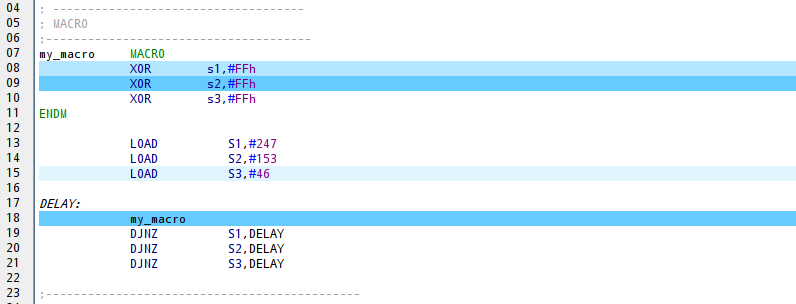
\includegraphics[width=\textwidth]{img/simulationcursor2.png}
            \caption{Simulation cursor}
        \end{figure}

    \clearpage
    \subsection{List of macros, breakpoints and bookmarks}
        For better orientation in what are you actually doing, MDS provides some additional tools located on the right
        panel, this includes List of Macros, List of Breakpoints, and List of Bookmarks.

        \begin{table}[h!]
            \begin{tabular}{ccc}
                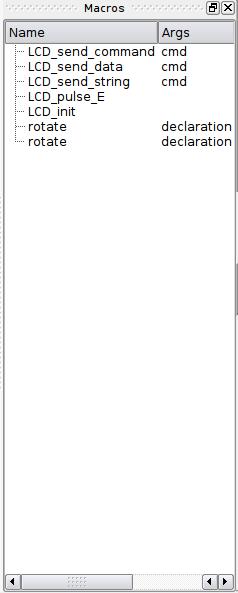
\includegraphics[width=.3\textwidth]{img/listmacros.png}
                    &
                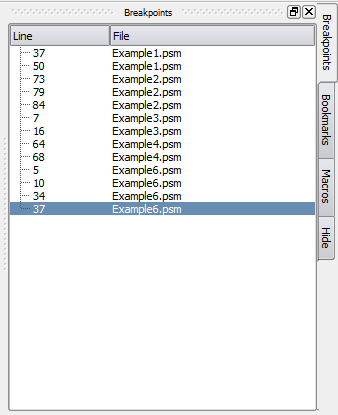
\includegraphics[width=.3\textwidth]{img/listbreakpoints.png}
                    &
                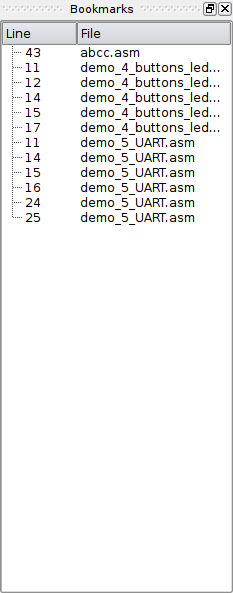
\includegraphics[width=.3\textwidth]{img/listbookmarks.png}
                \\ Macros & Breakpoints & Bookmarks
            \end{tabular}
        \end{table}


    \subsection{Modes of simulation}
        The simulator can operate three different modes:

        \begin{figure}[h!]
            \centering
            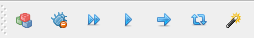
\includegraphics[width=.4\textwidth]{img/simulation_panel.png}
            \caption{Simulator toolbar.}
        \end{figure}

        \begin{description}
            \item [Step]
                Step by step simulation, executes only one instruction when invoked, no matter how many machine cycles
                it will take (this does not apply for macro-instruction, in that case each instruction of the macro is
                executed separately).
            \item [Animation]
                Similar to the step mode but in a loop, instructions are executed one after another until stopped on
                user request, or by a simulator waring message.
            \item [Run]
                Run is generally the same as animation but much faster, GUI is not updated so often, and changes in the
                registers, ports, etc. are not shown until the run is halted.
        \end{description}
